\documentclass[12pt]{article}

\usepackage[utf8]{inputenc}
\usepackage{latexsym,amsfonts,amssymb,amsthm,amsmath}
\usepackage{float}

\setlength{\parindent}{0in}
\setlength{\oddsidemargin}{0in}
\setlength{\textwidth}{6.5in}
\setlength{\textheight}{8.8in}
\setlength{\topmargin}{0in}
\setlength{\headheight}{18pt}
\usepackage{graphicx}
\usepackage{tikz}

\usepackage{hyperref}
\hypersetup{
    colorlinks=true,
    linkcolor=blue,
    filecolor=magenta,      
    urlcolor=cyan,
    pdftitle={Overleaf Example},
    pdfpagemode=FullScreen,
}

\urlstyle{same}

\usepackage{caption}
\DeclareCaptionFormat{citation}{%
  \ifx\captioncitation\relax\relax\else
    \captioncitation\par
  \fi
  #1#2#3\par}
\newcommand*\setcaptioncitation[1]{\def\captioncitation{\textit{Source:}~#1}}
\let\captioncitation\relax
\captionsetup{format=citation,justification=centering}

\title{MATH1034OL1 Pre-Calculus Mathematics Notes from Sections 5.2, 5.3 (Friday)}
\author{Elijah Renner}

\begin{document}

\maketitle

\vspace{0.5in}

\tableofcontents

\section{Compound Interest and the Natural Base}

For an initial amount \(P\), interest rate \(r\), compounding rate per time period \(t\), and time periods elapsed \(t\), we define the final amount \(A\) as\\

\[A=P\left(1+\frac{r}{n}\right)^{nt}\]\

If the compounding is continuous, meaning it's calculate infinitely many times in a given compounding period, the base is \(e\approx2.718\). Let's derive \(e\):\\

\[e=\lim_{x\to \infty}\left(1+\frac{1}{n}\right)^{1\cdot n}\]\

Hence, to calculate the new amount given an initial amount \(P\) after \(t\) time periods with interest rate \(r\), we use \(A=Pe^{rt}\)\\

For \(P=1000\), \(t=3\), and \(r=13\%\): \(A=1000e^{0.13\cdot 3}\approx1,476.98\)\\

\section{Logarithms}

\begin{figure}[H]
	\centering
	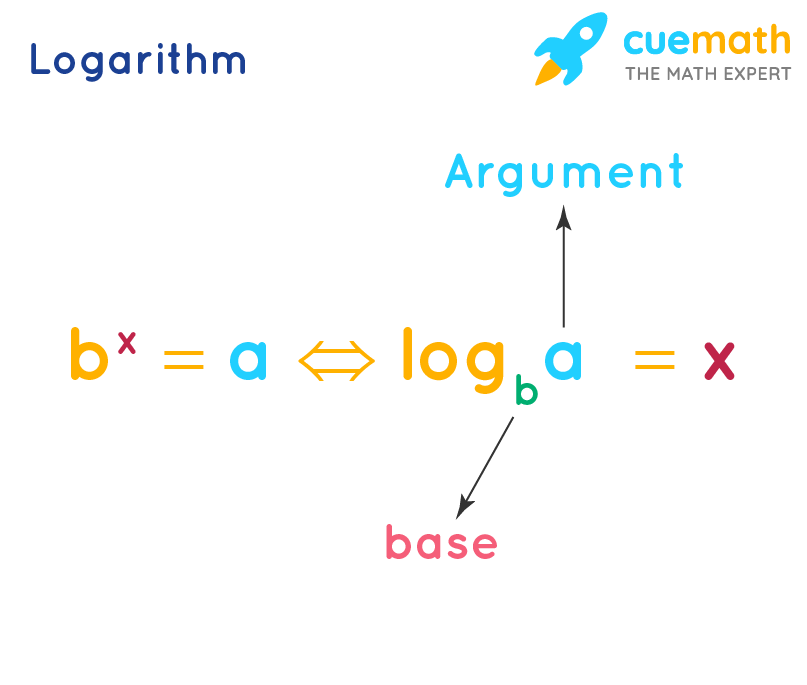
\includegraphics[scale=0.6]{logs.png}
	\caption{Credit: \url{https://www.cuemath.com/log-formulas/}}
\end{figure}

In plain language: the value of a logarithm is the power the base must be raised to in order to get the argument.\\

Logarithms are also the inverses of exponential functions. This means that for \(f(x)=b^x\), \(f^{-1}(x)=\log_bx\). Given this property, we know that a an exponential function and its corresponding inverse logarithmic function will reflect over the line \(y=x\):\\

\begin{figure}[H]
	\centering
	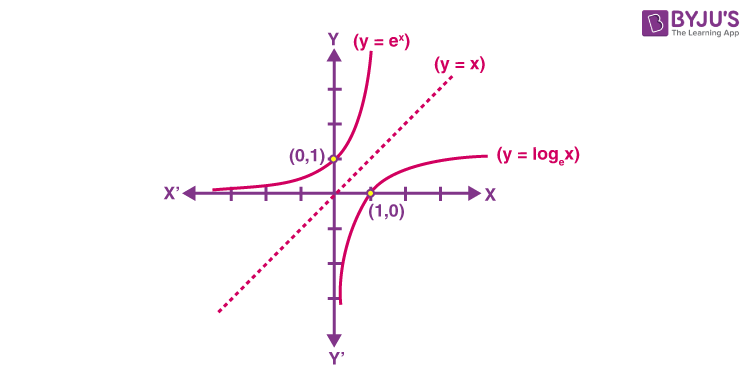
\includegraphics[scale=0.5]{inv.png}
	\caption{Credit: \url{https://byjus.com/maths/exponential-and-logarithmic-functions/}}
\end{figure}

Here are the rules to find the inverse of a logarithmic or exponential function:\\

\begin{figure}[H]
	\centering
	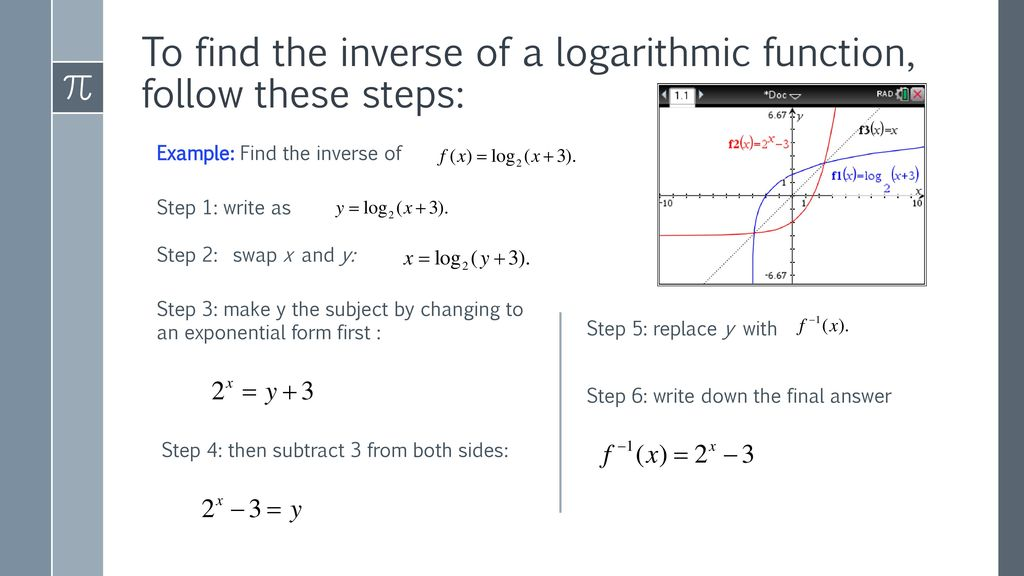
\includegraphics[scale=1.75]{loginv.jpg}
	\caption{Credit: \url{https://slideplayer.com/slide/12938368/}}
\end{figure}

\begin{figure}[H]
	\centering
	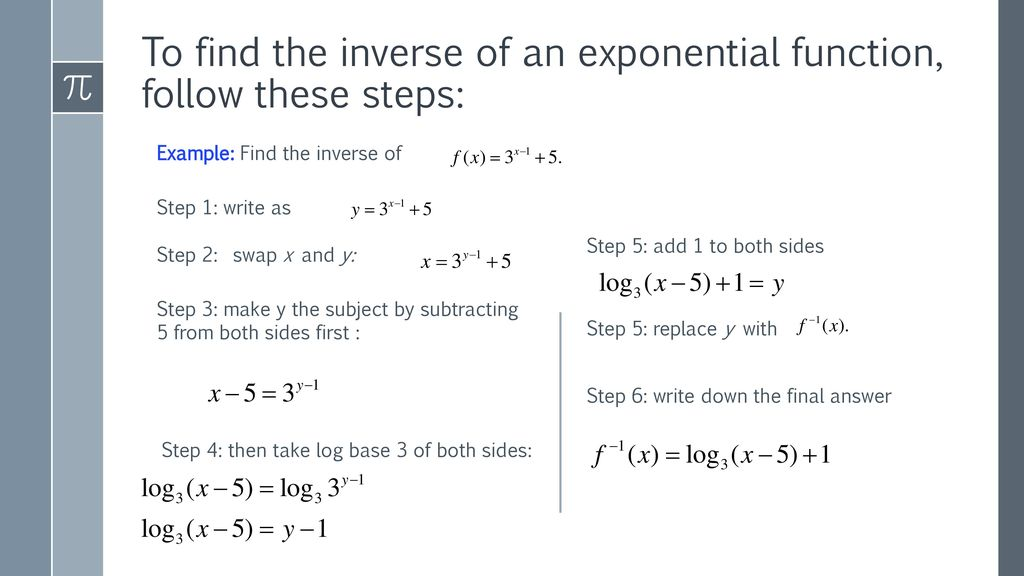
\includegraphics[scale=1.75]{expinv.jpg}
	\caption{Credit: \url{https://slideplayer.com/slide/12938368/}}
\end{figure}


We didn't discuss logarithmic graphs in class, but here are some important properties to understand:\\

\begin{figure}[H]
	\centering
	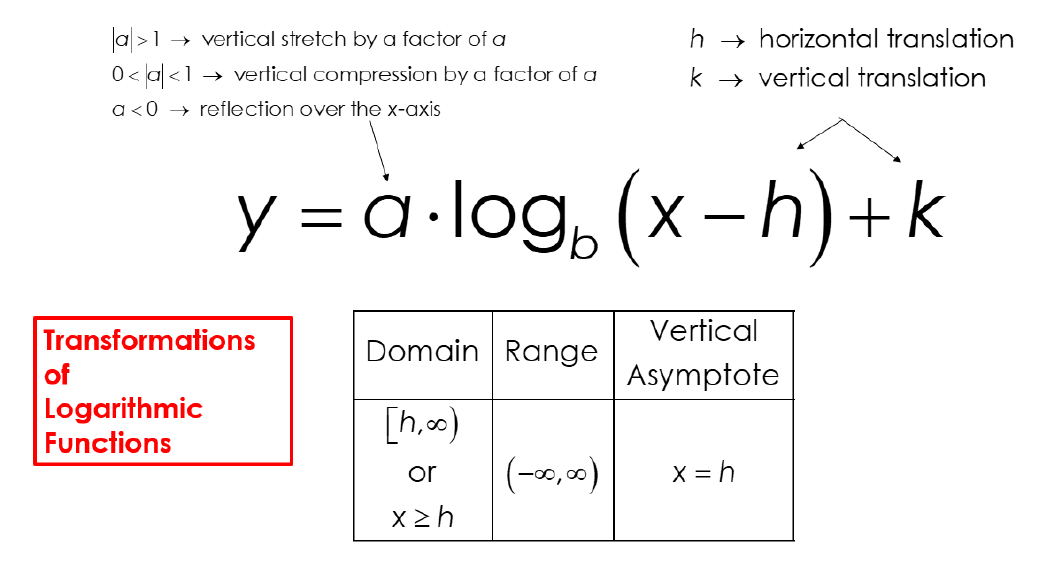
\includegraphics[scale=.45]{loggraph.png}
	\caption{Credit: \url{https://goodsifyet.shop/product_details/7113278.html}}
\end{figure}

There exists an asymptote at \(x=h\) because logarithmic functions may not have an argument less than 0. Similarly, they also may not have a negative base.\\

There are some rules for logarithms, too:\\

\begin{figure}[H]
	\centering
	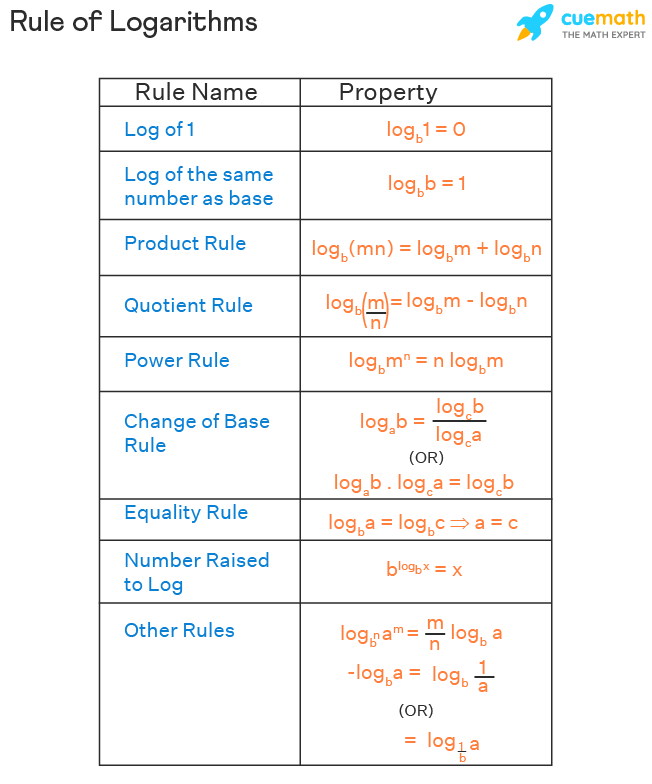
\includegraphics[scale=.52]{logrules.png}
	\caption{Credit: \url{https://www.cuemath.com/algebra/log-rules/}}
\end{figure}

\section{Fraction Exponents}

\[x^{\frac{a}{b}}=\sqrt[\leftroot{-2}\uproot{2}b]{x^a}=\left(\sqrt[\leftroot{-2}\uproot{2}b]{x}\right)^a\]

\end{document}